\documentclass{article}
\usepackage{iclr2026_conference,times}
%%%%% NEW MATH DEFINITIONS %%%%%

\usepackage{amsmath,amsfonts,bm}

% Mark sections of captions for referring to divisions of figures
\newcommand{\figleft}{{\em (Left)}}
\newcommand{\figcenter}{{\em (Center)}}
\newcommand{\figright}{{\em (Right)}}
\newcommand{\figtop}{{\em (Top)}}
\newcommand{\figbottom}{{\em (Bottom)}}
\newcommand{\captiona}{{\em (a)}}
\newcommand{\captionb}{{\em (b)}}
\newcommand{\captionc}{{\em (c)}}
\newcommand{\captiond}{{\em (d)}}

% Highlight a newly defined term
\newcommand{\newterm}[1]{{\bf #1}}


% Figure reference, lower-case.
\def\figref#1{figure~\ref{#1}}
% Figure reference, capital. For start of sentence
\def\Figref#1{Figure~\ref{#1}}
\def\twofigref#1#2{figures \ref{#1} and \ref{#2}}
\def\quadfigref#1#2#3#4{figures \ref{#1}, \ref{#2}, \ref{#3} and \ref{#4}}
% Section reference, lower-case.
\def\secref#1{section~\ref{#1}}
% Section reference, capital.
\def\Secref#1{Section~\ref{#1}}
% Reference to two sections.
\def\twosecrefs#1#2{sections \ref{#1} and \ref{#2}}
% Reference to three sections.
\def\secrefs#1#2#3{sections \ref{#1}, \ref{#2} and \ref{#3}}
% Reference to an equation, lower-case.
\def\eqref#1{equation~\ref{#1}}
% Reference to an equation, upper case
\def\Eqref#1{Equation~\ref{#1}}
% A raw reference to an equation---avoid using if possible
\def\plaineqref#1{\ref{#1}}
% Reference to a chapter, lower-case.
\def\chapref#1{chapter~\ref{#1}}
% Reference to an equation, upper case.
\def\Chapref#1{Chapter~\ref{#1}}
% Reference to a range of chapters
\def\rangechapref#1#2{chapters\ref{#1}--\ref{#2}}
% Reference to an algorithm, lower-case.
\def\algref#1{algorithm~\ref{#1}}
% Reference to an algorithm, upper case.
\def\Algref#1{Algorithm~\ref{#1}}
\def\twoalgref#1#2{algorithms \ref{#1} and \ref{#2}}
\def\Twoalgref#1#2{Algorithms \ref{#1} and \ref{#2}}
% Reference to a part, lower case
\def\partref#1{part~\ref{#1}}
% Reference to a part, upper case
\def\Partref#1{Part~\ref{#1}}
\def\twopartref#1#2{parts \ref{#1} and \ref{#2}}

\def\ceil#1{\lceil #1 \rceil}
\def\floor#1{\lfloor #1 \rfloor}
\def\1{\bm{1}}
\newcommand{\train}{\mathcal{D}}
\newcommand{\valid}{\mathcal{D_{\mathrm{valid}}}}
\newcommand{\test}{\mathcal{D_{\mathrm{test}}}}

\def\eps{{\epsilon}}


% Random variables
\def\reta{{\textnormal{$\eta$}}}
\def\ra{{\textnormal{a}}}
\def\rb{{\textnormal{b}}}
\def\rc{{\textnormal{c}}}
\def\rd{{\textnormal{d}}}
\def\re{{\textnormal{e}}}
\def\rf{{\textnormal{f}}}
\def\rg{{\textnormal{g}}}
\def\rh{{\textnormal{h}}}
\def\ri{{\textnormal{i}}}
\def\rj{{\textnormal{j}}}
\def\rk{{\textnormal{k}}}
\def\rl{{\textnormal{l}}}
% rm is already a command, just don't name any random variables m
\def\rn{{\textnormal{n}}}
\def\ro{{\textnormal{o}}}
\def\rp{{\textnormal{p}}}
\def\rq{{\textnormal{q}}}
\def\rr{{\textnormal{r}}}
\def\rs{{\textnormal{s}}}
\def\rt{{\textnormal{t}}}
\def\ru{{\textnormal{u}}}
\def\rv{{\textnormal{v}}}
\def\rw{{\textnormal{w}}}
\def\rx{{\textnormal{x}}}
\def\ry{{\textnormal{y}}}
\def\rz{{\textnormal{z}}}

% Random vectors
\def\rvepsilon{{\mathbf{\epsilon}}}
\def\rvtheta{{\mathbf{\theta}}}
\def\rva{{\mathbf{a}}}
\def\rvb{{\mathbf{b}}}
\def\rvc{{\mathbf{c}}}
\def\rvd{{\mathbf{d}}}
\def\rve{{\mathbf{e}}}
\def\rvf{{\mathbf{f}}}
\def\rvg{{\mathbf{g}}}
\def\rvh{{\mathbf{h}}}
\def\rvu{{\mathbf{i}}}
\def\rvj{{\mathbf{j}}}
\def\rvk{{\mathbf{k}}}
\def\rvl{{\mathbf{l}}}
\def\rvm{{\mathbf{m}}}
\def\rvn{{\mathbf{n}}}
\def\rvo{{\mathbf{o}}}
\def\rvp{{\mathbf{p}}}
\def\rvq{{\mathbf{q}}}
\def\rvr{{\mathbf{r}}}
\def\rvs{{\mathbf{s}}}
\def\rvt{{\mathbf{t}}}
\def\rvu{{\mathbf{u}}}
\def\rvv{{\mathbf{v}}}
\def\rvw{{\mathbf{w}}}
\def\rvx{{\mathbf{x}}}
\def\rvy{{\mathbf{y}}}
\def\rvz{{\mathbf{z}}}

% Elements of random vectors
\def\erva{{\textnormal{a}}}
\def\ervb{{\textnormal{b}}}
\def\ervc{{\textnormal{c}}}
\def\ervd{{\textnormal{d}}}
\def\erve{{\textnormal{e}}}
\def\ervf{{\textnormal{f}}}
\def\ervg{{\textnormal{g}}}
\def\ervh{{\textnormal{h}}}
\def\ervi{{\textnormal{i}}}
\def\ervj{{\textnormal{j}}}
\def\ervk{{\textnormal{k}}}
\def\ervl{{\textnormal{l}}}
\def\ervm{{\textnormal{m}}}
\def\ervn{{\textnormal{n}}}
\def\ervo{{\textnormal{o}}}
\def\ervp{{\textnormal{p}}}
\def\ervq{{\textnormal{q}}}
\def\ervr{{\textnormal{r}}}
\def\ervs{{\textnormal{s}}}
\def\ervt{{\textnormal{t}}}
\def\ervu{{\textnormal{u}}}
\def\ervv{{\textnormal{v}}}
\def\ervw{{\textnormal{w}}}
\def\ervx{{\textnormal{x}}}
\def\ervy{{\textnormal{y}}}
\def\ervz{{\textnormal{z}}}

% Random matrices
\def\rmA{{\mathbf{A}}}
\def\rmB{{\mathbf{B}}}
\def\rmC{{\mathbf{C}}}
\def\rmD{{\mathbf{D}}}
\def\rmE{{\mathbf{E}}}
\def\rmF{{\mathbf{F}}}
\def\rmG{{\mathbf{G}}}
\def\rmH{{\mathbf{H}}}
\def\rmI{{\mathbf{I}}}
\def\rmJ{{\mathbf{J}}}
\def\rmK{{\mathbf{K}}}
\def\rmL{{\mathbf{L}}}
\def\rmM{{\mathbf{M}}}
\def\rmN{{\mathbf{N}}}
\def\rmO{{\mathbf{O}}}
\def\rmP{{\mathbf{P}}}
\def\rmQ{{\mathbf{Q}}}
\def\rmR{{\mathbf{R}}}
\def\rmS{{\mathbf{S}}}
\def\rmT{{\mathbf{T}}}
\def\rmU{{\mathbf{U}}}
\def\rmV{{\mathbf{V}}}
\def\rmW{{\mathbf{W}}}
\def\rmX{{\mathbf{X}}}
\def\rmY{{\mathbf{Y}}}
\def\rmZ{{\mathbf{Z}}}

% Elements of random matrices
\def\ermA{{\textnormal{A}}}
\def\ermB{{\textnormal{B}}}
\def\ermC{{\textnormal{C}}}
\def\ermD{{\textnormal{D}}}
\def\ermE{{\textnormal{E}}}
\def\ermF{{\textnormal{F}}}
\def\ermG{{\textnormal{G}}}
\def\ermH{{\textnormal{H}}}
\def\ermI{{\textnormal{I}}}
\def\ermJ{{\textnormal{J}}}
\def\ermK{{\textnormal{K}}}
\def\ermL{{\textnormal{L}}}
\def\ermM{{\textnormal{M}}}
\def\ermN{{\textnormal{N}}}
\def\ermO{{\textnormal{O}}}
\def\ermP{{\textnormal{P}}}
\def\ermQ{{\textnormal{Q}}}
\def\ermR{{\textnormal{R}}}
\def\ermS{{\textnormal{S}}}
\def\ermT{{\textnormal{T}}}
\def\ermU{{\textnormal{U}}}
\def\ermV{{\textnormal{V}}}
\def\ermW{{\textnormal{W}}}
\def\ermX{{\textnormal{X}}}
\def\ermY{{\textnormal{Y}}}
\def\ermZ{{\textnormal{Z}}}

% Vectors
\def\vzero{{\bm{0}}}
\def\vone{{\bm{1}}}
\def\vmu{{\bm{\mu}}}
\def\vtheta{{\bm{\theta}}}
\def\va{{\bm{a}}}
\def\vb{{\bm{b}}}
\def\vc{{\bm{c}}}
\def\vd{{\bm{d}}}
\def\ve{{\bm{e}}}
\def\vf{{\bm{f}}}
\def\vg{{\bm{g}}}
\def\vh{{\bm{h}}}
\def\vi{{\bm{i}}}
\def\vj{{\bm{j}}}
\def\vk{{\bm{k}}}
\def\vl{{\bm{l}}}
\def\vm{{\bm{m}}}
\def\vn{{\bm{n}}}
\def\vo{{\bm{o}}}
\def\vp{{\bm{p}}}
\def\vq{{\bm{q}}}
\def\vr{{\bm{r}}}
\def\vs{{\bm{s}}}
\def\vt{{\bm{t}}}
\def\vu{{\bm{u}}}
\def\vv{{\bm{v}}}
\def\vw{{\bm{w}}}
\def\vx{{\bm{x}}}
\def\vy{{\bm{y}}}
\def\vz{{\bm{z}}}

% Elements of vectors
\def\evalpha{{\alpha}}
\def\evbeta{{\beta}}
\def\evepsilon{{\epsilon}}
\def\evlambda{{\lambda}}
\def\evomega{{\omega}}
\def\evmu{{\mu}}
\def\evpsi{{\psi}}
\def\evsigma{{\sigma}}
\def\evtheta{{\theta}}
\def\eva{{a}}
\def\evb{{b}}
\def\evc{{c}}
\def\evd{{d}}
\def\eve{{e}}
\def\evf{{f}}
\def\evg{{g}}
\def\evh{{h}}
\def\evi{{i}}
\def\evj{{j}}
\def\evk{{k}}
\def\evl{{l}}
\def\evm{{m}}
\def\evn{{n}}
\def\evo{{o}}
\def\evp{{p}}
\def\evq{{q}}
\def\evr{{r}}
\def\evs{{s}}
\def\evt{{t}}
\def\evu{{u}}
\def\evv{{v}}
\def\evw{{w}}
\def\evx{{x}}
\def\evy{{y}}
\def\evz{{z}}

% Matrix
\def\mA{{\bm{A}}}
\def\mB{{\bm{B}}}
\def\mC{{\bm{C}}}
\def\mD{{\bm{D}}}
\def\mE{{\bm{E}}}
\def\mF{{\bm{F}}}
\def\mG{{\bm{G}}}
\def\mH{{\bm{H}}}
\def\mI{{\bm{I}}}
\def\mJ{{\bm{J}}}
\def\mK{{\bm{K}}}
\def\mL{{\bm{L}}}
\def\mM{{\bm{M}}}
\def\mN{{\bm{N}}}
\def\mO{{\bm{O}}}
\def\mP{{\bm{P}}}
\def\mQ{{\bm{Q}}}
\def\mR{{\bm{R}}}
\def\mS{{\bm{S}}}
\def\mT{{\bm{T}}}
\def\mU{{\bm{U}}}
\def\mV{{\bm{V}}}
\def\mW{{\bm{W}}}
\def\mX{{\bm{X}}}
\def\mY{{\bm{Y}}}
\def\mZ{{\bm{Z}}}
\def\mBeta{{\bm{\beta}}}
\def\mPhi{{\bm{\Phi}}}
\def\mLambda{{\bm{\Lambda}}}
\def\mSigma{{\bm{\Sigma}}}

% Tensor
\DeclareMathAlphabet{\mathsfit}{\encodingdefault}{\sfdefault}{m}{sl}
\SetMathAlphabet{\mathsfit}{bold}{\encodingdefault}{\sfdefault}{bx}{n}
\newcommand{\tens}[1]{\bm{\mathsfit{#1}}}
\def\tA{{\tens{A}}}
\def\tB{{\tens{B}}}
\def\tC{{\tens{C}}}
\def\tD{{\tens{D}}}
\def\tE{{\tens{E}}}
\def\tF{{\tens{F}}}
\def\tG{{\tens{G}}}
\def\tH{{\tens{H}}}
\def\tI{{\tens{I}}}
\def\tJ{{\tens{J}}}
\def\tK{{\tens{K}}}
\def\tL{{\tens{L}}}
\def\tM{{\tens{M}}}
\def\tN{{\tens{N}}}
\def\tO{{\tens{O}}}
\def\tP{{\tens{P}}}
\def\tQ{{\tens{Q}}}
\def\tR{{\tens{R}}}
\def\tS{{\tens{S}}}
\def\tT{{\tens{T}}}
\def\tU{{\tens{U}}}
\def\tV{{\tens{V}}}
\def\tW{{\tens{W}}}
\def\tX{{\tens{X}}}
\def\tY{{\tens{Y}}}
\def\tZ{{\tens{Z}}}


% Graph
\def\gA{{\mathcal{A}}}
\def\gB{{\mathcal{B}}}
\def\gC{{\mathcal{C}}}
\def\gD{{\mathcal{D}}}
\def\gE{{\mathcal{E}}}
\def\gF{{\mathcal{F}}}
\def\gG{{\mathcal{G}}}
\def\gH{{\mathcal{H}}}
\def\gI{{\mathcal{I}}}
\def\gJ{{\mathcal{J}}}
\def\gK{{\mathcal{K}}}
\def\gL{{\mathcal{L}}}
\def\gM{{\mathcal{M}}}
\def\gN{{\mathcal{N}}}
\def\gO{{\mathcal{O}}}
\def\gP{{\mathcal{P}}}
\def\gQ{{\mathcal{Q}}}
\def\gR{{\mathcal{R}}}
\def\gS{{\mathcal{S}}}
\def\gT{{\mathcal{T}}}
\def\gU{{\mathcal{U}}}
\def\gV{{\mathcal{V}}}
\def\gW{{\mathcal{W}}}
\def\gX{{\mathcal{X}}}
\def\gY{{\mathcal{Y}}}
\def\gZ{{\mathcal{Z}}}

% Sets
\def\sA{{\mathbb{A}}}
\def\sB{{\mathbb{B}}}
\def\sC{{\mathbb{C}}}
\def\sD{{\mathbb{D}}}
% Don't use a set called E, because this would be the same as our symbol
% for expectation.
\def\sF{{\mathbb{F}}}
\def\sG{{\mathbb{G}}}
\def\sH{{\mathbb{H}}}
\def\sI{{\mathbb{I}}}
\def\sJ{{\mathbb{J}}}
\def\sK{{\mathbb{K}}}
\def\sL{{\mathbb{L}}}
\def\sM{{\mathbb{M}}}
\def\sN{{\mathbb{N}}}
\def\sO{{\mathbb{O}}}
\def\sP{{\mathbb{P}}}
\def\sQ{{\mathbb{Q}}}
\def\sR{{\mathbb{R}}}
\def\sS{{\mathbb{S}}}
\def\sT{{\mathbb{T}}}
\def\sU{{\mathbb{U}}}
\def\sV{{\mathbb{V}}}
\def\sW{{\mathbb{W}}}
\def\sX{{\mathbb{X}}}
\def\sY{{\mathbb{Y}}}
\def\sZ{{\mathbb{Z}}}

% Entries of a matrix
\def\emLambda{{\Lambda}}
\def\emA{{A}}
\def\emB{{B}}
\def\emC{{C}}
\def\emD{{D}}
\def\emE{{E}}
\def\emF{{F}}
\def\emG{{G}}
\def\emH{{H}}
\def\emI{{I}}
\def\emJ{{J}}
\def\emK{{K}}
\def\emL{{L}}
\def\emM{{M}}
\def\emN{{N}}
\def\emO{{O}}
\def\emP{{P}}
\def\emQ{{Q}}
\def\emR{{R}}
\def\emS{{S}}
\def\emT{{T}}
\def\emU{{U}}
\def\emV{{V}}
\def\emW{{W}}
\def\emX{{X}}
\def\emY{{Y}}
\def\emZ{{Z}}
\def\emSigma{{\Sigma}}

% entries of a tensor
% Same font as tensor, without \bm wrapper
\newcommand{\etens}[1]{\mathsfit{#1}}
\def\etLambda{{\etens{\Lambda}}}
\def\etA{{\etens{A}}}
\def\etB{{\etens{B}}}
\def\etC{{\etens{C}}}
\def\etD{{\etens{D}}}
\def\etE{{\etens{E}}}
\def\etF{{\etens{F}}}
\def\etG{{\etens{G}}}
\def\etH{{\etens{H}}}
\def\etI{{\etens{I}}}
\def\etJ{{\etens{J}}}
\def\etK{{\etens{K}}}
\def\etL{{\etens{L}}}
\def\etM{{\etens{M}}}
\def\etN{{\etens{N}}}
\def\etO{{\etens{O}}}
\def\etP{{\etens{P}}}
\def\etQ{{\etens{Q}}}
\def\etR{{\etens{R}}}
\def\etS{{\etens{S}}}
\def\etT{{\etens{T}}}
\def\etU{{\etens{U}}}
\def\etV{{\etens{V}}}
\def\etW{{\etens{W}}}
\def\etX{{\etens{X}}}
\def\etY{{\etens{Y}}}
\def\etZ{{\etens{Z}}}

% The true underlying data generating distribution
\newcommand{\pdata}{p_{\rm{data}}}
% The empirical distribution defined by the training set
\newcommand{\ptrain}{\hat{p}_{\rm{data}}}
\newcommand{\Ptrain}{\hat{P}_{\rm{data}}}
% The model distribution
\newcommand{\pmodel}{p_{\rm{model}}}
\newcommand{\Pmodel}{P_{\rm{model}}}
\newcommand{\ptildemodel}{\tilde{p}_{\rm{model}}}
% Stochastic autoencoder distributions
\newcommand{\pencode}{p_{\rm{encoder}}}
\newcommand{\pdecode}{p_{\rm{decoder}}}
\newcommand{\precons}{p_{\rm{reconstruct}}}

\newcommand{\laplace}{\mathrm{Laplace}} % Laplace distribution

\newcommand{\E}{\mathbb{E}}
\newcommand{\Ls}{\mathcal{L}}
\newcommand{\R}{\mathbb{R}}
\newcommand{\emp}{\tilde{p}}
\newcommand{\lr}{\alpha}
\newcommand{\reg}{\lambda}
\newcommand{\rect}{\mathrm{rectifier}}
\newcommand{\softmax}{\mathrm{softmax}}
\newcommand{\sigmoid}{\sigma}
\newcommand{\softplus}{\zeta}
\newcommand{\KL}{D_{\mathrm{KL}}}
\newcommand{\Var}{\mathrm{Var}}
\newcommand{\standarderror}{\mathrm{SE}}
\newcommand{\Cov}{\mathrm{Cov}}
% Wolfram Mathworld says $L^2$ is for function spaces and $\ell^2$ is for vectors
% But then they seem to use $L^2$ for vectors throughout the site, and so does
% wikipedia.
\newcommand{\normlzero}{L^0}
\newcommand{\normlone}{L^1}
\newcommand{\normltwo}{L^2}
\newcommand{\normlp}{L^p}
\newcommand{\normmax}{L^\infty}

\newcommand{\parents}{Pa} % See usage in notation.tex. Chosen to match Daphne's book.

\DeclareMathOperator*{\argmax}{arg\,max}
\DeclareMathOperator*{\argmin}{arg\,min}

\DeclareMathOperator{\sign}{sign}
\DeclareMathOperator{\Tr}{Tr}
\let\ab\allowbreak


\usepackage[utf8]{inputenc}
\usepackage[T1]{fontenc}
\usepackage{hyperref}
\usepackage{url}
\usepackage{booktabs}
\usepackage{graphicx}
\usepackage{xcolor}
\usepackage{amsmath}

\title{Error Analysis of LLMs on Romanian Polysemantic Crossword Clues:\\
What the Hints Actually Buy}

\author{Supplementary analysis for PolyCross / ThemCross}

\newif\ifllmic\llmictrue
\newcommand{\poly}{\textsc{PolyCross}}
\newcommand{\them}{\textsc{ThemCross}}
\newcommand{\tabsize}{\small\setlength{\tabcolsep}{3.2pt}}

\begin{document}
\maketitle

\begin{abstract}
We re-examine the solving results of four LLMs (Granite-4.0-small, Llama-3.3-70B, gpt-oss-120B and
Claude Opus 4.8) on \poly{} (polysemantic clues) and \them{} (straight thematic clues) under seven
hinting regimes, together with the Romanian base model LLMic-v2-3B under the five regimes a base
model can be prompted for. We (i)~rescore every model on the same 3000 \poly{} items that Claude was
evaluated on, (ii)~replace case-insensitive exact match with a diacritic-insensitive match, and
(iii)~decompose accuracy by how much of the answer the hint gives away. Three findings change how
the headline numbers should be read. First, strict matching penalised the open models by up to
10~points, and the apparent loss from chain-of-thought (v4 vs.\ v3) was almost entirely a diacritic
artifact. Second, at the four-letter prefix hint 44\% of items have their answer fully spelled out by
the hint; restricted to items where letters remain hidden, \poly{} accuracy drops by 10--18 points
for the stronger models, and on answers with three or more hidden letters it stays near 50\%.
Third, weaker models lose a large share of items simply by ignoring the hint, whereas the stronger
models' residual errors are hint-compliant words with the wrong meaning --- the failure mode the
benchmark is designed to expose. The Romanian base model is weakest on both counts: it rarely
respects the length hint, and where letters remain hidden it solves about 5\% of \poly{} items.
\end{abstract}

% --------------------------------------------------------------------------
\section{Setup and rescoring}
\label{sec:setup}

\paragraph{Items.} \poly{} is scored on the 3000-item sample \texttt{polycross\_sample3000.json}
(seed 42, answers of at least three letters) that Claude Opus 4.8 was evaluated on; \them{} on its
1148 items with answers of at least three letters. The three open models were originally run on the
full $\sim$26k-item \poly{} corpus; we align their predictions to the sample by (clue, answer). An item
missing from a run (a request that failed every retry) counts as wrong, so every cell has the same
denominator. The one run that did not exist, Llama-3.3-70B on \poly{} at $k{=}4$, was produced on
the 3000 sample with the same prompt (59.8\%; the 52.3\% quoted in the rebuttal has no
corresponding result file, and the new run uses the current RITS deployment of the model). Table~\ref{tab:continuity} shows that the sample tracks the
full corpus to within about one point, so conclusions from the sample transfer.

\paragraph{Conditions.} v1: clue only; v2: clue + answer length; v3: length + the first $k\in\{1,2,3,4\}$
letters; v4: v3 with chain-of-thought (answer in brackets); v5: length hint, reason in English and
answer in Romanian. When the answer has at most $k$ letters the prefix hint contains the whole answer.

% Flip to \llmictrue once the LLMic results (run_llmic.sh) are in data/results;
% the tables and figures pick the model up automatically.
\ifllmic
\paragraph{A Romanian base model.} LLMic-v2-3B (B\u{a}doiu et al., 2025; arXiv:2501.07721) is a 3B-parameter
Romanian--English \emph{foundation} model without instruction tuning or a chat template, so it cannot
follow the JSON instruction prompts above. We evaluate it with few-shot \emph{completion} prompts that
carry the same three worked examples and the same hint wording as v1--v3, ending in
``R\u{a}spuns:''; the answer is its greedy continuation up to the first newline. v4 and v5 rely on
following instructions and have no base-model analogue, so they are omitted (``--'' in the tables).
The prompts must be tokenized with the model's own \texttt{tokenizer.json}: the default
\texttt{transformers}~5 tokenizer class drops its newline pre-tokenizer, and with it the model
produces no usable answers (0.0\% on \poly{} v1).
\fi

\paragraph{Diacritic-insensitive scoring.} Gold answers are written without diacritics
(\textsc{zambila}), while models frequently answer with them (\textsc{zambilă}), and the original
metric counted those as errors. We now compare both strings after Unicode NFD decomposition, removal
of combining marks, upper-casing and removal of non-letters (which also neutralises the lower-case
intersection markers in \poly{} answers such as \textsc{pRAF}). We report this as \emph{accuracy}
throughout; Table~\ref{tab:strict} in the appendix gives the strict numbers.

\begin{table}[!htb]
\centering\tabsize
\caption{Accuracy (\%, diacritic-insensitive) on the common item sets. Best per column in bold.
Len = length hint; Tr.\ = translate (v5). 95\% bootstrap intervals are at most $\pm1.8$ points on
\poly{} and $\pm3.0$ on \them{}.}
\label{tab:accuracy}
\begin{tabular}{lrrrrrrrrrrr}
\toprule
 & \multicolumn{2}{c}{} & \multicolumn{4}{c}{v3: length + prefix} & \multicolumn{4}{c}{v4: v3 + CoT} & v5 \\
\cmidrule(lr){4-7}\cmidrule(lr){8-11}
Model & \multicolumn{1}{c}{No} & \multicolumn{1}{c}{Len} & $k{=}1$ & $k{=}2$ & $k{=}3$ & $k{=}4$ & $k{=}1$ & $k{=}2$ & $k{=}3$ & $k{=}4$ & \multicolumn{1}{c}{Tr.} \\
\midrule
\multicolumn{12}{l}{\textit{PolyCross}} \\
\quad Granite-4.0-small & 0.6 & 1.1 & 5.1 & 11.8 & 28.7 & 40.8 & 3.5 & 7.0 & 20.3 & 32.7 & 0.7 \\
\quad Llama-3.3-70B & 2.5 & 4.1 & 12.3 & 25.0 & 43.3 & 59.8 & 14.1 & 25.4 & 46.9 & 58.8 & 4.6 \\
\quad gpt-oss-120B & 3.8 & 7.9 & 23.0 & 39.7 & 61.4 & 76.6 & 23.5 & 40.0 & 62.9 & 76.3 & 8.0 \\
\quad Claude Opus 4.8 & \textbf{5.2} & \textbf{8.7} & \textbf{28.4} & \textbf{50.7} & \textbf{75.8} & \textbf{85.6} & \textbf{29.6} & \textbf{50.7} & \textbf{75.9} & \textbf{86.1} & \textbf{8.8} \\
\quad LLMic-v2-3B & 0.4 & 0.1 & 1.5 & 3.9 & 22.8 & 43.6 & -- & -- & -- & -- & -- \\
\midrule
\multicolumn{12}{l}{\textit{ThemCross}} \\
\quad Granite-4.0-small & 11.1 & 13.6 & 20.1 & 27.2 & 40.4 & 54.4 & 11.4 & 15.4 & 19.3 & 30.1 & 9.8 \\
\quad Llama-3.3-70B & 30.9 & 35.2 & 46.1 & 52.7 & 63.9 & 74.3 & 48.1 & 53.3 & 63.8 & 73.8 & 39.4 \\
\quad gpt-oss-120B & 35.2 & 46.6 & 56.9 & 64.4 & 77.6 & 87.5 & 58.9 & 65.6 & 76.5 & 88.2 & 47.6 \\
\quad Claude Opus 4.8 & \textbf{59.1} & \textbf{65.1} & \textbf{83.0} & \textbf{88.3} & \textbf{92.8} & \textbf{95.5} & \textbf{83.0} & \textbf{88.3} & \textbf{93.5} & \textbf{95.6} & \textbf{73.5} \\
\quad LLMic-v2-3B & 4.7 & 3.7 & 7.4 & 11.9 & 26.7 & 47.3 & -- & -- & -- & -- & -- \\
\bottomrule
\end{tabular}

\end{table}

\paragraph{Effect of rescoring.} Table~\ref{tab:delta} lists the change per cell. It is small for
Claude Opus 4.8, whose answers are nearly always diacritic-free (the exception is v5 on \them{},
+5.7), and substantial for the open
models, above all under the bracketed-answer prompts: gpt-oss-120B gains 9.8 points on \poly{} v4
$k{=}4$ (66.5$\rightarrow$76.3) and 9.1 on \them{} v4 $k{=}1$. Two conclusions of the original
analysis change as a result (\S\ref{sec:prompts}): chain-of-thought no longer hurts the stronger
models, and the translation prompt is no worse than the plain length hint.

\begin{figure}[!htb]
\centering
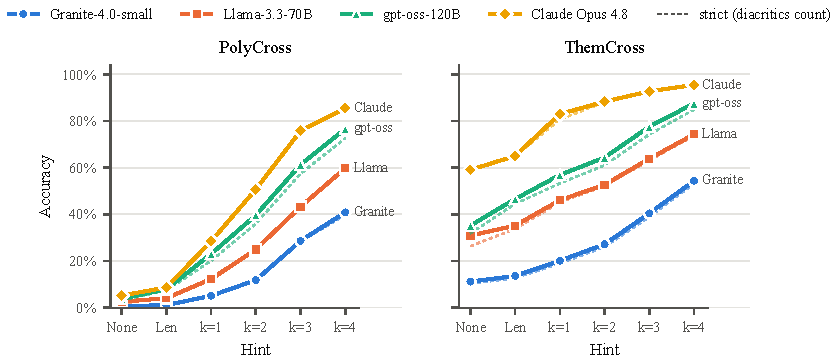
\includegraphics[width=\linewidth]{figures/accuracy_ladder.pdf}
\caption{Accuracy along the hint ladder (v1, v2, v3 $k{=}1..4$). Solid: diacritic-insensitive;
dashed: strict. The gap between the two lines is the diacritic penalty; it is widest for gpt-oss-120B.}
\label{fig:ladder}
\end{figure}

% --------------------------------------------------------------------------
\section{How much of the answer does the hint give away?}
\label{sec:hints}

Accuracy rises steeply with $k$ (Figure~\ref{fig:ladder}), and on \poly{} the four-letter hint takes
Claude Opus 4.8 from 8.7\% to 85.6\%. How much of this reflects clue understanding? We split items
by the number of letters the hint leaves hidden, $|a|-k$ (Table~\ref{tab:strata},
Figure~\ref{fig:strata}).

\paragraph{Fully revealed answers.} At $k{=}4$, 44.0\% of \poly{} and 44.7\% of \them{} items have
$|a|\le 4$, so the hint \emph{is} the answer. Claude Opus 4.8 and gpt-oss-120B score 97--100\% on
these, as expected. Granite-4.0-small and Llama-3.3-70B do not: they return the given string on only
57--69\% and 64--86\% of these items respectively, typically by producing a longer word that starts
with the hint. This is a hint-following failure, not a reasoning one.
\ifllmic LLMic-v2-3B copies the hint on 87\% ($k{=}3$) and 94\% ($k{=}4$) of these \poly{} items,
more often than Granite or Llama, and they account for almost all of its accuracy: its 43.6\% at
$k{=}4$, which puts it above Granite-4.0-small, falls to 4.2\% on the remaining items, the lowest of
all models.\fi

\paragraph{Informative-hint accuracy.} Restricted to items with $|a|>k$, \poly{} accuracy at $k{=}4$
is 75.1\% for Claude Opus 4.8 (vs.\ 85.6\% overall) and 58.5\% for gpt-oss-120B (vs.\ 76.6\%). With
three or more letters hidden it falls to 52.9\% and 46.1\%. On \them{} the same restriction costs
Claude less than 3 points: straight definitions remain solvable when the hint leaves most of the word
open, polysemantic ones do not. We recommend reporting informative-hint accuracy alongside overall
accuracy for all prefix conditions.

\begin{figure}[!htb]
\centering
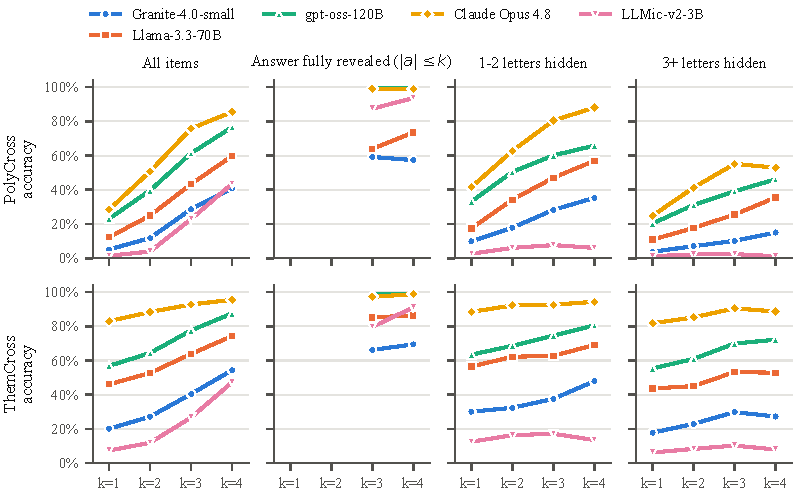
\includegraphics[width=\linewidth]{figures/strata.pdf}
\caption{v3 accuracy by how many answer letters the hint leaves hidden. The ``fully revealed''
panel only exists for $k\ge3$ because all answers have at least three letters.}
\label{fig:strata}
\end{figure}

\begin{table}[!htb]
\centering\tabsize
\caption{v3 accuracy (\%) by the number of letters the hint leaves hidden. Gray: share of items in
the stratum at each $k$.}
\label{tab:strata}
\begin{tabular}{llrrrr}
\toprule
Items & Model & $k{=}1$ & $k{=}2$ & $k{=}3$ & $k{=}4$ \\
\midrule
\multicolumn{6}{l}{\textbf{PolyCross}} \\
\multicolumn{2}{l}{\textit{$|a| \le k$ (answer fully revealed)}} & \textcolor{gray}{0\%} & \textcolor{gray}{0\%} & \textcolor{gray}{21\%} & \textcolor{gray}{44\%} \\
 & Granite-4.0-small & -- & -- & 59.2 & 57.4 \\
 & Llama-3.3-70B & -- & -- & 63.9 & 73.5 \\
 & gpt-oss-120B & -- & -- & 99.7 & 99.5 \\
 & Claude Opus 4.8 & -- & -- & 99.1 & 98.9 \\
\addlinespace
\multicolumn{2}{l}{\textit{$|a|-k \in \{1,2\}$}} & \textcolor{gray}{21\%} & \textcolor{gray}{44\%} & \textcolor{gray}{45\%} & \textcolor{gray}{35\%} \\
 & Granite-4.0-small & 9.9 & 17.9 & 28.3 & 35.3 \\
 & Llama-3.3-70B & 17.4 & 34.2 & 47.1 & 56.9 \\
 & gpt-oss-120B & 33.1 & 50.5 & 60.1 & 65.8 \\
 & Claude Opus 4.8 & 41.6 & 62.8 & 80.5 & 88.1 \\
\addlinespace
\multicolumn{2}{l}{\textit{$|a|-k \ge 3$}} & \textcolor{gray}{79\%} & \textcolor{gray}{56\%} & \textcolor{gray}{34\%} & \textcolor{gray}{21\%} \\
 & Granite-4.0-small & 3.8 & 7.0 & 10.2 & 15.0 \\
 & Llama-3.3-70B & 10.9 & 17.7 & 25.5 & 35.5 \\
 & gpt-oss-120B & 20.3 & 31.1 & 39.1 & 46.1 \\
 & Claude Opus 4.8 & 24.9 & 41.3 & 55.2 & 52.9 \\
\addlinespace
\multicolumn{2}{l}{\textit{$|a|>k$ (informative)}} & \textcolor{gray}{100\%} & \textcolor{gray}{100\%} & \textcolor{gray}{79\%} & \textcolor{gray}{56\%} \\
 & Granite-4.0-small & 5.1 & 11.8 & 20.4 & 27.8 \\
 & Llama-3.3-70B & 12.3 & 25.0 & 37.7 & 49.0 \\
 & gpt-oss-120B & 23.0 & 39.7 & 51.0 & 58.5 \\
 & Claude Opus 4.8 & 28.4 & 50.7 & 69.5 & 75.1 \\
\addlinespace
\midrule
\multicolumn{6}{l}{\textbf{ThemCross}} \\
\multicolumn{2}{l}{\textit{$|a| \le k$ (answer fully revealed)}} & \textcolor{gray}{0\%} & \textcolor{gray}{0\%} & \textcolor{gray}{19\%} & \textcolor{gray}{45\%} \\
 & Granite-4.0-small & -- & -- & 66.2 & 69.4 \\
 & Llama-3.3-70B & -- & -- & 85.2 & 86.4 \\
 & gpt-oss-120B & -- & -- & 99.1 & 99.0 \\
 & Claude Opus 4.8 & -- & -- & 97.2 & 98.8 \\
\addlinespace
\multicolumn{2}{l}{\textit{$|a|-k \in \{1,2\}$}} & \textcolor{gray}{19\%} & \textcolor{gray}{45\%} & \textcolor{gray}{48\%} & \textcolor{gray}{40\%} \\
 & Granite-4.0-small & 30.1 & 32.4 & 37.6 & 47.9 \\
 & Llama-3.3-70B & 56.5 & 62.2 & 62.7 & 69.1 \\
 & gpt-oss-120B & 63.4 & 68.6 & 74.5 & 80.6 \\
 & Claude Opus 4.8 & 88.4 & 92.2 & 92.6 & 94.3 \\
\addlinespace
\multicolumn{2}{l}{\textit{$|a|-k \ge 3$}} & \textcolor{gray}{81\%} & \textcolor{gray}{55\%} & \textcolor{gray}{33\%} & \textcolor{gray}{15\%} \\
 & Granite-4.0-small & 17.8 & 23.0 & 29.8 & 27.3 \\
 & Llama-3.3-70B & 43.7 & 45.0 & 53.3 & 52.8 \\
 & gpt-oss-120B & 55.4 & 60.9 & 69.9 & 72.2 \\
 & Claude Opus 4.8 & 81.8 & 85.2 & 90.5 & 88.6 \\
\addlinespace
\multicolumn{2}{l}{\textit{$|a|>k$ (informative)}} & \textcolor{gray}{100\%} & \textcolor{gray}{100\%} & \textcolor{gray}{81\%} & \textcolor{gray}{55\%} \\
 & Granite-4.0-small & 20.1 & 27.2 & 34.4 & 42.2 \\
 & Llama-3.3-70B & 46.1 & 52.7 & 58.9 & 64.6 \\
 & gpt-oss-120B & 56.9 & 64.4 & 72.6 & 78.3 \\
 & Claude Opus 4.8 & 83.0 & 88.3 & 91.7 & 92.8 \\
\addlinespace
\bottomrule
\end{tabular}

\end{table}

\paragraph{How constraining is the hint?} A complementary view counts how many words from the
crossword vocabulary (the union of all answers in both full corpora, 11.9k types) fit the length and
prefix. Figure~\ref{fig:candidates} pools v3 over $k$, excluding fully revealed items. On \poly{},
accuracy falls monotonically with the number of candidates for every model: Claude Opus 4.8 goes from
78\% when a single vocabulary word fits to 22\% when more than 100 do. On \them{} its curve is nearly
flat (95\%$\rightarrow$81\%). The contrast is the clearest signature of the benchmark's premise: for
polysemantic clues, a large part of the prefix-hint gain comes from narrowing the candidate set rather
than from resolving the clue.

\begin{figure}[!htb]
\centering
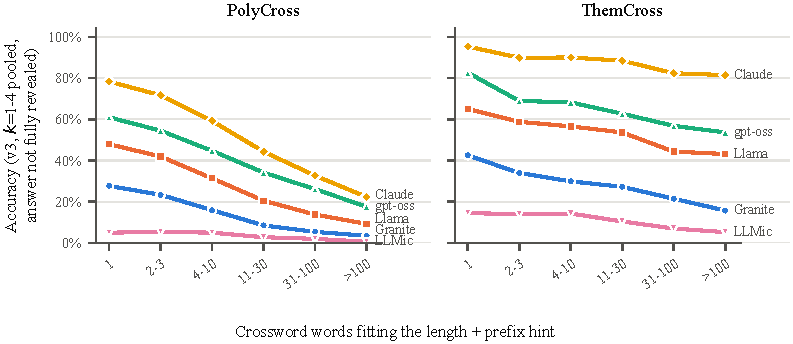
\includegraphics[width=\linewidth]{figures/candidates.pdf}
\caption{v3 accuracy against the number of crossword-vocabulary words consistent with the hint.}
\label{fig:candidates}
\end{figure}

\paragraph{Answer length.} Figure~\ref{fig:heatmap} breaks accuracy down by answer length. On \poly{}
without prefix hints, accuracy is in single digits at every length. Once letters are given, short
answers are solved first and long answers lag: at $k{=}4$ Claude Opus 4.8 solves 91\% of five-letter
but only 34\% of 10+-letter \poly{} answers. On \them{} length matters much less.

\begin{figure}[!htb]
\centering
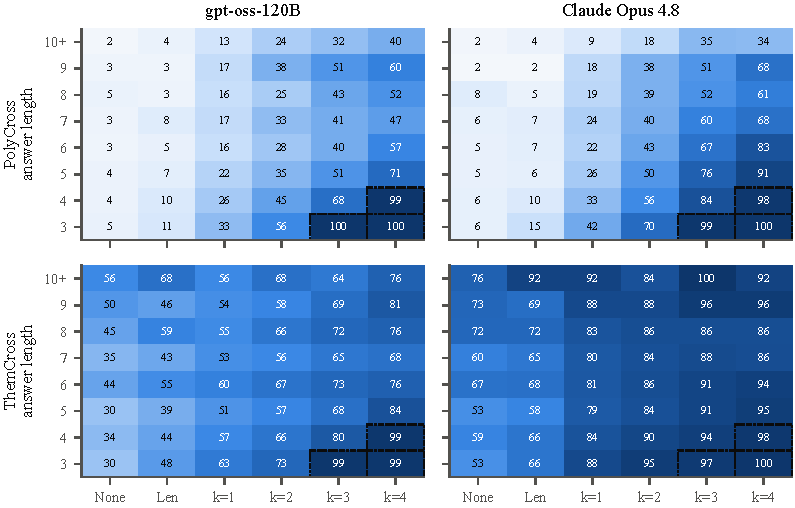
\includegraphics[width=\linewidth]{figures/length_heatmap.pdf}
\caption{Accuracy (\%) by answer length and hint level for the two strongest models. Dotted cells:
the hint contains the whole answer.}
\label{fig:heatmap}
\end{figure}

% --------------------------------------------------------------------------
\section{What kinds of errors remain?}
\label{sec:errors}

We assign each wrong prediction to the first matching category: \emph{no answer} (empty or
unparseable); \emph{wrong length} (the length was given but not respected); \emph{wrong prefix}
(given letters not respected); \emph{one letter off} (edit distance 1 from the answer, counted only
when at least two letters were hidden, since otherwise every wrong completion is trivially one edit
away); and \emph{other word, fits hint}. Figure~\ref{fig:errors} shows the composition.

\begin{figure}[!htb]
\centering
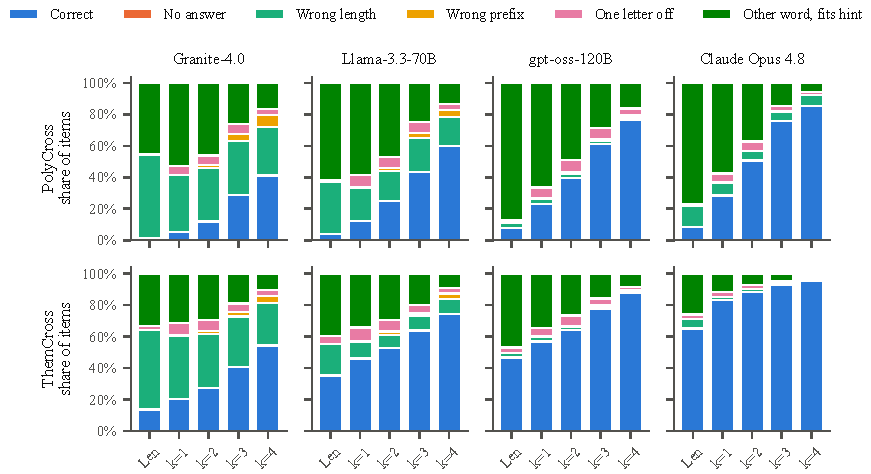
\includegraphics[width=\linewidth]{figures/errors.pdf}
\caption{Share of all items that are correct or fall into each error category, per model and hint
level.}
\label{fig:errors}
\end{figure}

\paragraph{Hint violations dominate for the weaker models.} Granite-4.0-small gives an answer of the
wrong length on 31--53\% of \poly{} items at every hint level, and Llama-3.3-70B on 19--33\%.
Among answered items, gpt-oss-120B and Claude Opus 4.8 respect both the length and the prefix
92--99\% of the time (Table~\ref{tab:compliance} in the appendix).
\ifllmic LLMic-v2-3B keeps the given prefix on 91--100\% of items but the given length on only
17--45\% on \poly{} (19--51\% on \them{}): the few-shot completion conveys the letters, but the base
model does not treat the stated length as a constraint. Wrong length is therefore its dominant error
at every hint level.\fi An exception is Claude Opus 4.8 at
v2 on \poly{}, which violates the length on 13.1\% of items, more than gpt-oss-120B (3.4\%): without
letters to anchor it, it sometimes prefers a semantically apt word of the wrong length.

\paragraph{The stronger models fail on meaning, not on form.} For gpt-oss-120B and Claude Opus 4.8,
almost all remaining errors are hint-compliant words, which is the failure mode the benchmark targets:
the model settles on a reading of the clue that yields a plausible word of the right shape, but not
the intended one. Near misses (one letter off) are a small share throughout, so partial credit would
change little. Table~\ref{tab:examples} lists examples. They also show that many \poly{} answers are
not dictionary words but crossword fragments or multi-word strings (\textsc{atot}, \textsc{tria},
\textsc{vincusifon}, \textsc{ineldeaur}, ``3 cuv.''), which a model cannot reach without
the crossword convention that licenses them.

% --------------------------------------------------------------------------
\section{Difficulty across models and hint levels}
\label{sec:difficulty}

\paragraph{Agreement.} Figure~\ref{fig:agreement} counts how many of the models solve each
item, over the conditions every model was run on (v1--v3\ifllmic; five models including
LLMic-v2-3B\fi). Without prefix hints, 91.3\% (v1) and 85.1\% (v2) of \poly{} items are solved by no
model at all, versus 36.0\% and 28.6\% on \them{}. Items solved by exactly one model are overwhelmingly
Claude's: at v3 $k{=}2$ it solves 445 \poly{} items that no other model does, against 205 for
gpt-oss-120B. Claude Opus 4.8 beats gpt-oss-120B significantly (exact McNemar, $p<0.01$) in every
\poly{} condition with a prefix hint and in every \them{} condition, but not at v2 or v5 on \poly{}
($p=0.22$, $0.16$), where both are below 9\%.

\begin{figure}[!htb]
\centering
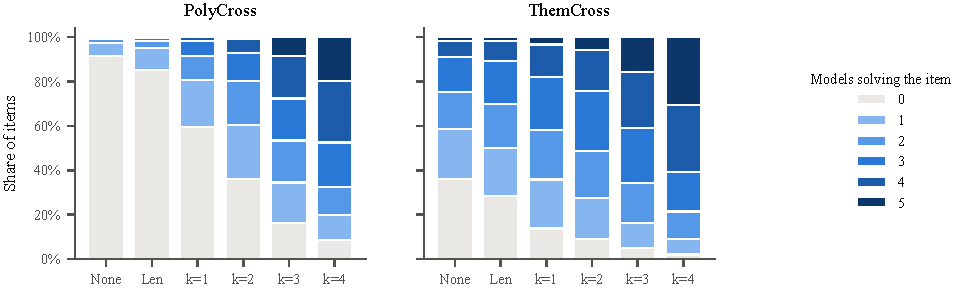
\includegraphics[width=\linewidth]{figures/agreement.pdf}
\caption{Share of items solved by none, some or all of the models, per hint level (v1--v3).}
\label{fig:agreement}
\end{figure}

\paragraph{When is an item first solved?} Along the ladder v2 $\rightarrow$ v3 $k{=}1..4$
(Table~\ref{tab:progression}), most \them{} items that Claude Opus 4.8 solves are solved with the
length hint alone (67\% of the items it ever solves), whereas on \poly{} they are spread across $k{=}1$--3. The ladder is not
monotone: 8.6\% of \poly{} items are solved by Claude at some $k$ and missed again at a larger $k$,
and 5--12\% for the other models (6--21\% across models on \them{}). Part of the gain from one hint level to the next is therefore
sampling variance rather than information, which argues for reporting intervals
(Table~\ref{tab:accuracy} caption) and paired tests rather than point differences.

\begin{table}[!htb]
\centering\tabsize
\caption{The hint level at which each item is first solved (\% of items), items never solved, and
items solved at some level but missed at a larger one.}
\label{tab:progression}
\begin{tabular}{llrrrrrrr}
\toprule
 & & \multicolumn{5}{c}{First solved at} & & \\
\cmidrule(lr){3-7}
Dataset & Model & Len & $k{=}1$ & $k{=}2$ & $k{=}3$ & $k{=}4$ & Never & Lost later \\
\midrule
PolyCross & Granite-4.0-small & 1.1 & 4.5 & 8.4 & 19.1 & 16.3 & 50.5 & 12.3 \\
 & Llama-3.3-70B & 4.1 & 8.7 & 14.9 & 21.4 & 17.1 & 33.9 & 10.9 \\
 & gpt-oss-120B & 7.9 & 16.0 & 18.6 & 22.7 & 15.3 & 19.6 & 8.9 \\
 & Claude Opus 4.8 & 8.7 & 20.7 & 24.3 & 24.7 & 11.0 & 10.6 & 8.6 \\
\midrule
ThemCross & Granite-4.0-small & 13.6 & 9.9 & 11.1 & 14.6 & 14.6 & 36.1 & 20.5 \\
 & Llama-3.3-70B & 35.2 & 15.3 & 10.9 & 11.8 & 11.4 & 15.4 & 21.3 \\
 & gpt-oss-120B & 46.6 & 14.7 & 8.5 & 11.9 & 9.2 & 9.0 & 12.5 \\
 & Claude Opus 4.8 & 65.1 & 19.1 & 6.8 & 3.7 & 2.9 & 2.4 & 6.2 \\
\bottomrule
\end{tabular}

\end{table}

% --------------------------------------------------------------------------
\section{Prompting strategies revisited}
\label{sec:prompts}

\paragraph{Chain-of-thought (v4 vs.\ v3).} Under strict scoring, v4 appeared to hurt gpt-oss-120B
by up to 6 points at $k{=}4$ on \poly{}. After rescoring the two are within 2 points at every $k$ for
gpt-oss-120B and Claude Opus 4.8, and no difference is significant at $p<0.01$ (Table~\ref{tab:cot}).
The strict penalty came from the bracketed free-text answer, where models write diacritics more
often than in the JSON answer of v3. Chain-of-thought does help Llama-3.3-70B on \poly{} at $k{=}3$
(+3.6, $p<0.01$), and clearly hurts Granite-4.0-small (up to $-24$ points on \them{}), which often
fails to produce the bracketed answer in the right form.

\begin{table}[!htb]
\centering\tabsize
\caption{Accuracy difference v4 $-$ v3 (points). $^{*}$: exact McNemar $p<0.01$.}
\label{tab:cot}
\begin{tabular}{llrrrr}
\toprule
Dataset & Model & $k{=}1$ & $k{=}2$ & $k{=}3$ & $k{=}4$ \\
\midrule
PolyCross & Granite-4.0-small & -1.6$^{*}$ & -4.8$^{*}$ & -8.3$^{*}$ & -8.1$^{*}$ \\
 & Llama-3.3-70B & +1.9$^{*}$ & +0.4 & +3.6$^{*}$ & -1.0 \\
 & gpt-oss-120B & +0.4 & +0.4 & +1.5 & -0.3 \\
 & Claude Opus 4.8 & +1.2 & -0.0 & +0.1 & +0.5 \\
\midrule
ThemCross & Granite-4.0-small & -8.7$^{*}$ & -11.8$^{*}$ & -21.1$^{*}$ & -24.2$^{*}$ \\
 & Llama-3.3-70B & +2.0 & +0.6 & -0.1 & -0.5 \\
 & gpt-oss-120B & +2.0 & +1.2 & -1.1 & +0.6 \\
 & Claude Opus 4.8 & +0.0 & +0.0 & +0.7 & +0.2 \\
\bottomrule
\end{tabular}

\end{table}

\paragraph{Translation (v5 vs.\ v2).} Both prompts give only the length hint; v5 additionally asks the
model to reason in English. After rescoring, v5 matches v2 for gpt-oss-120B and Claude Opus 4.8 on
\poly{} and \emph{exceeds} it for Claude on \them{} (73.5 vs.\ 65.1; Table~\ref{tab:translation}).
The rate of answers outside the crossword vocabulary rises by at most 2 points under v5 for the
stronger models (and falls for Claude on \them{}), so we find no evidence that answers are lost in translating back to Romanian. The one clear failure is
Granite-4.0-small, which gives no usable answer on 21\% (\poly{}) and 28\% (\them{}) of v5 items.
The difficulty of polysemantic clues therefore lies in finding the intended sense, which translation
neither creates nor removes.

\begin{table}[!htb]
\centering\tabsize
\caption{Translate (v5) vs.\ length hint (v2), \%. No ans.: empty or unparseable. OOV (out of vocabulary): answered with a word that is not an
answer anywhere in either full corpus (an over-estimate because of inflected forms; compare columns
rather than read absolute values). Len.\ ok: answer has the given length.}
\label{tab:translation}
\begin{tabular}{llrrrrrrrr}
\toprule
 & & \multicolumn{2}{c}{Acc.} & \multicolumn{2}{c}{No ans.} & \multicolumn{2}{c}{OOV} & \multicolumn{2}{c}{Len.\ ok} \\
\cmidrule(lr){3-4}\cmidrule(lr){5-6}\cmidrule(lr){7-8}\cmidrule(lr){9-10}
Dataset & Model & v2 & v5 & v2 & v5 & v2 & v5 & v2 & v5 \\
\midrule
PolyCross & Granite-4.0-small & 1.1 & 0.7 & 0.4 & 20.6 & 72.3 & 71.5 & 47.1 & 38.6 \\
 & Llama-3.3-70B & 4.1 & 4.6 & 0.0 & 1.8 & 63.1 & 50.8 & 66.9 & 75.1 \\
 & gpt-oss-120B & 7.9 & 8.0 & 0.1 & 4.4 & 44.0 & 45.7 & 96.6 & 96.5 \\
 & Claude Opus 4.8 & 8.7 & 8.8 & 0.0 & 0.0 & 53.7 & 53.2 & 86.9 & 82.2 \\
\midrule
ThemCross & Granite-4.0-small & 13.6 & 9.8 & 0.3 & 27.8 & 68.2 & 69.8 & 49.3 & 41.0 \\
 & Llama-3.3-70B & 35.2 & 39.4 & 0.0 & 1.7 & 46.2 & 38.4 & 80.0 & 84.3 \\
 & gpt-oss-120B & 46.6 & 47.6 & 0.0 & 0.9 & 30.1 & 31.6 & 97.0 & 97.0 \\
 & Claude Opus 4.8 & 65.1 & 73.5 & 0.0 & 0.0 & 23.3 & 14.7 & 93.9 & 96.6 \\
\bottomrule
\end{tabular}

\end{table}

% --------------------------------------------------------------------------
\section{Takeaways}
\label{sec:takeaways}

\begin{enumerate}
\item \textbf{Score without diacritics.} Strict matching understated the open models by up to 10 points
      and produced two spurious conclusions (chain-of-thought and translation both appearing to hurt).
\item \textbf{Report informative-hint accuracy.} At $k{\ge}3$ a large fraction of items is solved by
      the hint alone. Accuracy on $|a|>k$, and on $|a|-k\ge3$, measures clue understanding far better.
\item \textbf{The \poly{}--\them{} gap survives every control.} With three or more letters hidden,
      Claude Opus 4.8 reaches 89\% on \them{} but 53\% on \poly{} at $k{=}4$; without prefix hints the
      gap is 54--65 points for Claude and 31--40 for gpt-oss-120B.
\item \textbf{Weaker models fail on form, stronger ones on meaning.} Hint violations explain much of the
      gap between Granite/Llama and the rest; the remaining errors of the strongest models are
      well-formed words with the wrong sense.\ifllmic{} The Romanian base model LLMic-v2-3B has the
      lowest informative-hint accuracy of all models in every condition, mainly because it ignores
      the length hint.\fi
\end{enumerate}

\clearpage
\appendix
\section{Additional tables}

\begin{table}[h]
\centering\tabsize
\caption{Strict accuracy (\%, case-insensitive exact match, diacritics count), as in the original
analysis but on the common item sets.}
\label{tab:strict}
\begin{tabular}{lrrrrrrrrrrr}
\toprule
 & \multicolumn{2}{c}{} & \multicolumn{4}{c}{v3: length + prefix} & \multicolumn{4}{c}{v4: v3 + CoT} & v5 \\
\cmidrule(lr){4-7}\cmidrule(lr){8-11}
Model & \multicolumn{1}{c}{No} & \multicolumn{1}{c}{Len} & $k{=}1$ & $k{=}2$ & $k{=}3$ & $k{=}4$ & $k{=}1$ & $k{=}2$ & $k{=}3$ & $k{=}4$ & \multicolumn{1}{c}{Tr.} \\
\midrule
\multicolumn{12}{l}{\textit{PolyCross}} \\
\quad Granite-4.0-small & 0.5 & 1.1 & 4.9 & 11.6 & 28.4 & 39.8 & 2.6 & 6.0 & 18.5 & 29.6 & 0.6 \\
\quad Llama-3.3-70B & 1.9 & 3.9 & 11.9 & 24.7 & 42.9 & 59.3 & 11.7 & 21.5 & 42.1 & 53.5 & 3.9 \\
\quad gpt-oss-120B & 3.2 & 7.4 & 20.1 & 36.0 & 57.4 & 72.7 & 18.5 & 32.5 & 53.7 & 66.5 & 6.5 \\
\quad Claude Opus 4.8 & \textbf{5.2} & \textbf{8.7} & \textbf{28.4} & \textbf{50.7} & \textbf{75.8} & \textbf{85.6} & \textbf{29.6} & \textbf{50.7} & \textbf{75.9} & \textbf{86.1} & \textbf{8.8} \\
\quad LLMic-v2-3B & 0.3 & 0.1 & 1.2 & 3.5 & 22.1 & 42.3 & -- & -- & -- & -- & -- \\
\midrule
\multicolumn{12}{l}{\textit{ThemCross}} \\
\quad Granite-4.0-small & 10.3 & 12.7 & 19.0 & 26.0 & 38.9 & 53.2 & 9.7 & 12.9 & 16.7 & 27.7 & 8.0 \\
\quad Llama-3.3-70B & 26.4 & 33.8 & 45.2 & 52.2 & 63.2 & 73.8 & 42.5 & 47.7 & 58.8 & 67.9 & 35.5 \\
\quad gpt-oss-120B & 31.9 & 44.5 & 53.3 & 61.1 & 74.3 & 84.9 & 49.8 & 56.9 & 69.3 & 85.0 & 39.3 \\
\quad Claude Opus 4.8 & \textbf{59.0} & \textbf{65.1} & \textbf{80.7} & \textbf{88.2} & \textbf{92.8} & \textbf{95.5} & \textbf{82.8} & \textbf{88.2} & \textbf{93.5} & \textbf{95.6} & \textbf{67.8} \\
\quad LLMic-v2-3B & 4.1 & 3.1 & 6.4 & 10.5 & 25.3 & 46.0 & -- & -- & -- & -- & -- \\
\bottomrule
\end{tabular}

\end{table}

\begin{table}[h]
\centering\tabsize
\caption{Change from rescoring: diacritic-insensitive minus strict accuracy (points).}
\label{tab:delta}
\begin{tabular}{lrrrrrrrrrrr}
\toprule
 & \multicolumn{2}{c}{} & \multicolumn{4}{c}{v3: length + prefix} & \multicolumn{4}{c}{v4: v3 + CoT} & v5 \\
\cmidrule(lr){4-7}\cmidrule(lr){8-11}
Model & \multicolumn{1}{c}{No} & \multicolumn{1}{c}{Len} & $k{=}1$ & $k{=}2$ & $k{=}3$ & $k{=}4$ & $k{=}1$ & $k{=}2$ & $k{=}3$ & $k{=}4$ & \multicolumn{1}{c}{Tr.} \\
\midrule
\multicolumn{12}{l}{\textit{PolyCross}} \\
\quad Granite-4.0-small & 0.1 & 0.0 & 0.2 & 0.2 & 0.2 & 1.0 & 0.8 & 1.0 & 1.8 & 3.1 & 0.1 \\
\quad Llama-3.3-70B & 0.6 & 0.1 & 0.4 & 0.2 & 0.4 & 0.5 & 2.4 & 3.9 & 4.8 & 5.3 & 0.7 \\
\quad gpt-oss-120B & 0.6 & 0.5 & 3.0 & 3.7 & 3.9 & 3.9 & 5.0 & 7.6 & 9.2 & 9.8 & 1.5 \\
\quad Claude Opus 4.8 & 0.0 & 0.0 & 0.0 & 0.0 & 0.0 & 0.0 & 0.0 & 0.0 & 0.0 & 0.0 & 0.1 \\
\quad LLMic-v2-3B & 0.1 & 0.0 & 0.2 & 0.4 & 0.7 & 1.2 & -- & -- & -- & -- & -- \\
\midrule
\multicolumn{12}{l}{\textit{ThemCross}} \\
\quad Granite-4.0-small & 0.9 & 0.9 & 1.1 & 1.1 & 1.5 & 1.1 & 1.7 & 2.5 & 2.6 & 2.4 & 1.7 \\
\quad Llama-3.3-70B & 4.5 & 1.4 & 0.9 & 0.5 & 0.7 & 0.5 & 5.6 & 5.6 & 5.0 & 5.8 & 3.9 \\
\quad gpt-oss-120B & 3.3 & 2.1 & 3.6 & 3.3 & 3.3 & 2.6 & 9.1 & 8.7 & 7.2 & 3.1 & 8.4 \\
\quad Claude Opus 4.8 & 0.1 & 0.0 & 2.3 & 0.2 & 0.0 & 0.0 & 0.2 & 0.1 & 0.0 & 0.0 & 5.7 \\
\quad LLMic-v2-3B & 0.6 & 0.5 & 1.0 & 1.4 & 1.4 & 1.3 & -- & -- & -- & -- & -- \\
\bottomrule
\end{tabular}

\end{table}

\begin{table}[h]
\centering\tabsize
\caption{The open models on \poly{}: full corpus (their original runs) vs.\ the 3000-item sample.
The Llama $k{=}4$ run exists only on the sample.}
\label{tab:continuity}
\begin{tabular}{llrrrr}
\toprule
 & & \multicolumn{2}{c}{Full corpus ($\sim$26k)} & \multicolumn{2}{c}{Sample (3000)} \\
\cmidrule(lr){3-4}\cmidrule(lr){5-6}
Model & Cond. & strict & no-diac. & strict & no-diac. \\
\midrule
Granite-4.0-small & No hint & 0.6 & 0.7 & 0.5 & 0.6 \\
Granite-4.0-small & Length & 1.1 & 1.1 & 1.1 & 1.1 \\
Granite-4.0-small & v3 k=2 & 11.7 & 12.0 & 11.6 & 11.8 \\
Granite-4.0-small & v3 k=4 & 39.7 & 40.5 & 39.8 & 40.8 \\
Granite-4.0-small & v4 k=4 & 29.2 & 32.4 & 29.6 & 32.7 \\
Granite-4.0-small & Translate & 0.6 & 0.7 & 0.6 & 0.7 \\
\addlinespace
Llama-3.3-70B & No hint & 1.7 & 2.2 & 1.9 & 2.5 \\
Llama-3.3-70B & Length & 3.5 & 3.6 & 3.9 & 4.1 \\
Llama-3.3-70B & v3 k=2 & 24.3 & 24.7 & 24.7 & 25.0 \\
Llama-3.3-70B & v4 k=4 & 55.2 & 60.4 & 53.5 & 58.8 \\
Llama-3.3-70B & Translate & 3.8 & 4.5 & 3.9 & 4.6 \\
\addlinespace
gpt-oss-120B & No hint & 2.8 & 3.4 & 3.2 & 3.8 \\
gpt-oss-120B & Length & 7.6 & 8.2 & 7.4 & 7.9 \\
gpt-oss-120B & v3 k=2 & 34.8 & 38.4 & 36.0 & 39.7 \\
gpt-oss-120B & v3 k=4 & 72.8 & 76.6 & 72.7 & 76.6 \\
gpt-oss-120B & v4 k=4 & 67.1 & 76.4 & 66.5 & 76.3 \\
gpt-oss-120B & Translate & 6.4 & 8.0 & 6.5 & 8.0 \\
\bottomrule
\end{tabular}

\end{table}

\begin{table}[h]
\centering\tabsize
\caption{Hint compliance among answered items (\%): answer has the given length (v2--v5), and the
given length and prefix (v3/v4).}
\label{tab:compliance}
\begin{tabular}{llrrrrrr}
\toprule
Dataset & Model & Length & v3 k=1 & v3 k=2 & v3 k=3 & v3 k=4 & Translate \\
\midrule
PolyCross & Granite-4.0-small & 47.1 & 63.6 & 63.9 & 61.2 & 61.4 & 38.6 \\
 & Llama-3.3-70B & 66.9 & 78.2 & 79.0 & 75.1 & 77.1 & 75.1 \\
 & gpt-oss-120B & 96.6 & 96.4 & 96.4 & 97.0 & 97.2 & 96.5 \\
 & Claude Opus 4.8 & 86.9 & 91.7 & 93.9 & 93.7 & 93.1 & 82.2 \\
 & LLMic-v2-3B & 16.8 & 18.3 & 20.5 & 27.5 & 44.9 & -- \\
\midrule
ThemCross & Granite-4.0-small & 49.3 & 59.4 & 63.7 & 64.7 & 68.9 & 41.0 \\
 & Llama-3.3-70B & 80.0 & 88.9 & 89.5 & 89.4 & 87.1 & 84.3 \\
 & gpt-oss-120B & 97.0 & 96.9 & 97.7 & 97.6 & 98.3 & 97.0 \\
 & Claude Opus 4.8 & 93.9 & 97.8 & 98.0 & 98.5 & 98.3 & 96.6 \\
 & LLMic-v2-3B & 19.1 & 24.2 & 27.8 & 33.2 & 49.5 & -- \\
\bottomrule
\end{tabular}

\end{table}

\begin{table}[h]
\centering\tabsize
\caption{Wrong answers at v3 $k{=}2$ on \poly{}, sampled at random per error category.}
\label{tab:examples}
\begin{tabular}{p{0.34\linewidth}lll}
\toprule
Clue & Answer & Prediction & Model \\
\midrule
\multicolumn{4}{l}{\textit{One letter off}} \\
Ultima rezervă de materie cenuşie & URNA & URMA & Claude Opus 4.8 \\
Rezultatul adunării & ATOT & ATOM & Claude Opus 4.8 \\
Animal... pentru tăiat de ocazie & LAMA & LADA & Claude Opus 4.8 \\
Implicată într-o afacere în pierdere & DATA & DANA & gpt-oss-120B \\
Impun măsuri restrictive pentru limitarea debordărilor & LIMITATIVI & LIMITATIVE & gpt-oss-120B \\
O fată care stă la tușă & VARA & VACA & gpt-oss-120B \\
\addlinespace
\multicolumn{4}{l}{\textit{Other word, fits hint}} \\
A avansa de la echipa mare & TRIA & TREC & Claude Opus 4.8 \\
Active pe perioada alegerilor & SITE & SIGL & Claude Opus 4.8 \\
Oglindiți în lumina adevărului & REALI & REDAT & Claude Opus 4.8 \\
Pornire cu violenţă & ARTAG & ARUNC & gpt-oss-120B \\
Ataşat naval & VAS & VAL & gpt-oss-120B \\
Nimb prețios pentru sanctitatea iubirii (3 cuv.) & INELDEAUR & IN INIMA TA & gpt-oss-120B \\
\addlinespace
\multicolumn{4}{l}{\textit{Wrong length}} \\
Iarba verde unde se iese cu grupul & PASCATOARE & PAJISTELE & Claude Opus 4.8 \\
Dă semne că se face rău & AVERTIZARE & AVERTIZEA & Claude Opus 4.8 \\
Disimularea unui om cu pretenții exagerate & INFUMURARE & INFATUARE & Claude Opus 4.8 \\
Tensiunea instalată pentru senzori de vibraţii & NELINISTE & NECESITA & gpt-oss-120B \\
Instalat din start printre favoriți & ATU & ATOP & gpt-oss-120B \\
Atac la persoană & MISTOCARIE & MISOGENIE & gpt-oss-120B \\
\addlinespace
\multicolumn{4}{l}{\textit{Wrong prefix}} \\
Substratul unui adevăr... pus la îndoială & VINCUSIFON & VERIDICITA & Claude Opus 4.8 \\
Precedent pentru noi & NEO & NOU & Claude Opus 4.8 \\
Odoare iubite de părinți (sing.) & ORAR & ODOR & Claude Opus 4.8 \\
Pune bazele înălţării & CTITOR & CIMENT & gpt-oss-120B \\
Rezultatul adunării & NOIAN & NUMAR & gpt-oss-120B \\
Concept generic de acțiune în scădere & IEFTINIRE & DIMINUARE & gpt-oss-120B \\
\addlinespace
\bottomrule
\end{tabular}

\end{table}

\end{document}
